% Module 5: Natural Language Processing - short assignment report
% Compile with XeLaTeX: latexmk -xelatex report.tex
\documentclass{article}

\PassOptionsToPackage{numbers,compress}{natbib}
\usepackage[final]{template22}
% Common packages
\usepackage[utf8]{inputenc} % allow utf-8 input
\usepackage[T1]{fontenc}    % use 8-bit T1 fonts
\usepackage{microtype}
\usepackage{times}
\usepackage{graphicx}
\usepackage{amsmath,amssymb,mathbbol}
% \usepackage{algorithmic}
% \usepackage[linesnumbered,ruled,vlined]{algorithm2e}
\usepackage{acronym}
\usepackage{enumitem}
\usepackage[pagebackref=true,breaklinks=true,colorlinks]{hyperref}
\usepackage{balance}
\usepackage{xspace}
\usepackage{setspace}
\usepackage[skip=3pt,font=small]{subcaption}
\usepackage[skip=3pt,font=small]{caption}
\usepackage[dvipsnames]{xcolor}
\usepackage[capitalise]{cleveref}
\usepackage{booktabs,tabularx,colortbl,multirow,array,makecell}
% \usepackage{overpic,wrapfig}

\usepackage{fancyhdr}
\hypersetup{pdfencoding=auto,colorlinks=true,allcolors=black}
\renewcommand{\headrulewidth}{0.5pt}
\renewcommand{\footrulewidth}{0pt}
\fancyhf{}
\fancyhead[C]{}
\fancyhead[C]{}
\fancyfoot[C]{\thepage}

% Handy shorthand
\makeatletter
\DeclareRobustCommand\onedot{\futurelet\@let@token\@onedot}
\def\@onedot{\ifx\@let@token.\else.\null\fi\xspace}
\def\eg{\emph{e.g}\onedot} 
\def\Eg{\emph{E.g}\onedot}
\def\ie{\emph{i.e}\onedot} 
\def\Ie{\emph{I.e}\onedot}
\def\cf{\emph{c.f}\onedot} 
\def\Cf{\emph{C.f}\onedot}
\def\etc{\emph{etc}\onedot} 
\def\vs{\emph{vs}\onedot}
\def\wrt{w.r.t\onedot} 
\def\dof{d.o.f\onedot}
\def\etal{\emph{et al}\onedot}
\makeatother

\definecolor{gray}{gray}{0.9}

% Handy math ops
\DeclareMathOperator*{\argmax}{arg\,max}
\DeclareMathOperator*{\argmin}{arg\,min}
\newcommand{\norm}[1]{\left\Vert #1 \right\Vert}

% % Spacing
\frenchspacing
% \medmuskip=2mu   % reduce spacing around binary operators
% \thickmuskip=3mu % reduce spacing around relational operators
% \setlength{\abovedisplayskip}{3pt}
% \setlength{\belowdisplayskip}{3pt}
% \setlength{\abovecaptionskip}{3pt}
% \setlength{\belowcaptionskip}{3pt}
\setlength\floatsep{0.5\baselineskip plus 3pt minus 2pt}
\setlength\textfloatsep{0.5\baselineskip plus 3pt minus 2pt}
\setlength\dbltextfloatsep{0.5\baselineskip plus 3pt minus 2pt}
\setlength\intextsep{0.5\baselineskip plus 3pt minus 2pt}

\makeatletter
\renewcommand{\paragraph}{%
  \@startsection{paragraph}{4}%
  {\z@}{0ex \@plus 0ex \@minus 0ex}{-1em}%
  {\hskip\parindent\normalfont\normalsize\bfseries}%
}
\makeatother

% Graphics path
\graphicspath{{figures/}}

% Clever references
\crefname{algorithm}{Alg.}{Algs.}
\Crefname{algorithm}{Algorithm}{Algorithms}
\crefname{section}{Sec.}{Secs.}
\Crefname{section}{Section}{Sections}
\crefname{table}{Tab.}{Tabs.}
\Crefname{table}{Table}{Tables}
\crefname{figure}{Fig.}{Fig.}
\Crefname{figure}{Figure}{Figure}

% Acronym
\acrodef{pku}[PKU]{Peking University}
\usepackage{tikz}
\usetikzlibrary{arrows.meta,positioning,calc}

\title{Belief Context Graph Feedback\\
for BrowseComp Agents}

\author{%
  Yuanze Lei \quad 2510124204\\
  Peking University
}

\begin{document}
\maketitle

\begin{abstract}
This report proposes a task-oriented research agent that uses the open-source
Belief Context Graph (BCG) as both an auditable memory and a feedback
controller. BCG incrementally turns tool calls, tool results, available
reasoning summaries, and intermediate conclusions into typed belief and
decision nodes with confidence, provenance, and relations. The agent then uses
the graph to identify one weak link on the path to its current answer and
intervenes through a bounded evidence-verification search. We specify the
integration path, the graph representation, the weak-link policy, and a
reproducible BrowseComp comparison. The report is a design for the full
assignment; it makes no claim of measured benchmark performance.
\end{abstract}

\section{Problem and Design Goals}\label{sec:problem}

BrowseComp requires a browsing agent to answer difficult factual questions
through multiple searches and source comparisons \citep{wei2025browsecomp}.
Long trajectories therefore contain several different kinds of state: search
queries, retrieved snippets, partial conclusions, contradictions, and the
eventual answer. Keeping every turn in the raw context is expensive, while
ordinary summarisation loses the provenance needed to audit an answer. A
vector-memory layer retrieves similar text but does not explicitly represent
which claim depends on which evidence or which claim is uncertain.

We use BCG as a belief-aware context layer \citep{bcg2026}. The important
direction is deliberately two-way. During execution, the agent emits events and
BCG records them as an evidence-grounded graph. Before the next model call, the
agent reads the graph, locates the weakest belief on the current reasoning
path, and may change its next action instead of merely carrying the graph as
passive history. The design goal is not to replace the agent's planner with a
graph. It is to expose the part of the agent state that is uncertain enough to
justify a targeted intervention.

\begin{figure}[t]
\centering
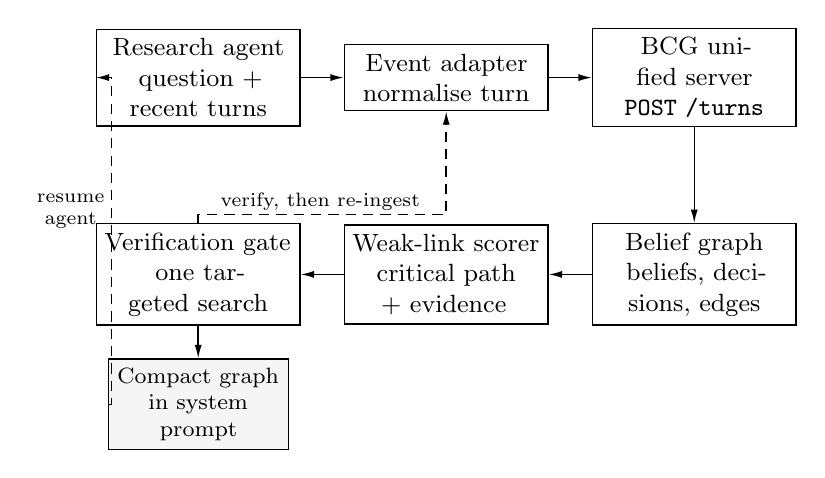
\begin{tikzpicture}[
  x=1cm,y=1cm,
  box/.style={draw=black,line width=0.5pt,fill=white,align=center,
    minimum height=0.82cm,text width=2.35cm,font=\small},
  smallbox/.style={draw=black,line width=0.45pt,fill=black!4,align=center,
    minimum height=0.64cm,text width=2.05cm,font=\footnotesize},
  arrow/.style={-{Latex[length=1.7mm,width=0.9mm]},draw=black,
    line width=0.55pt},
  dashedarrow/.style={-{Latex[length=1.7mm,width=0.9mm]},draw=black,
    line width=0.55pt,dash pattern=on 1.3mm off 0.9mm}
]
  \node[box] (agent) at (0,2.6) {Research agent\\question + recent turns};
  \node[box] (adapter) at (3.15,2.6) {Event adapter\\normalise turn};
  \node[box] (server) at (6.3,2.6) {BCG unified server\\\texttt{POST /turns}};
  \node[box] (graph) at (6.3,0.1) {Belief graph\\beliefs, decisions, edges};
  \node[box] (score) at (3.15,0.1) {Weak-link scorer\\critical path + evidence};
  \node[box] (gate) at (0,0.1) {Verification gate\\one targeted search};
  \node[smallbox] (prompt) at (0,-1.55) {Compact graph\\in system prompt};

  \draw[arrow] (agent) -- (adapter);
  \draw[arrow] (adapter) -- (server);
  \draw[arrow] (server) -- (graph);
  \draw[arrow] (graph) -- (score);
  \draw[arrow] (score) -- (gate);
  \draw[arrow] (gate) -- (prompt);
  \draw[dashedarrow] (prompt.west) -- (-1.1,-1.55) -- (-1.1,2.6)
    -- (agent.west);
  \draw[dashedarrow] (gate.north) -- (0,0.86) -- (3.15,0.86)
    -- (adapter.south);

  \node[font=\scriptsize,align=center] at (-1.62,0.9)
    {resume\\agent};
  \node[font=\scriptsize,align=center] at (1.55,1.02)
    {verify, then re-ingest};
\end{tikzpicture}
\caption{BCG is used as a feedback layer. The agent's completed turns are
recorded as a belief graph; a weak-link scorer reads the graph and either
injects a compact snapshot or requests one focused verification search. The
dashed path shows the new evidence returning to the graph.}
\label{fig:architecture}
\end{figure}

\section{BCG Integration and Graph Construction}\label{sec:integration}

\subsection{Service-level integration}

We use the BCG HTTP construction service rather than reimplementing its
extraction and confidence rules. The proposed implementation pins the current
BCG release, version 1.0.0, and the repository commit
\texttt{e00283e90e590346052819dd5ee6894e2601fb5d}. The service is started with
the \texttt{unified} backend:

\begin{center}
\small
\texttt{bcg construct server unified -{}-host 127.0.0.1 -{}-port 8848}
\end{center}

Each BrowseComp task is assigned a stable \texttt{problem\_id}. The adapter
normalises every completed event to a role-tagged turn and sends it to
\texttt{POST /turn}; consecutive tool results from one assistant message can be
sent to \texttt{POST /turns} as a batch. The final event sets
\texttt{is\_trajectory\_end}. The agent reads a snapshot with
\texttt{GET /graph?problem\_id=...}. The HTTP service keeps construction
concurrency and graph artifacts outside the agent process, which makes the
integration easier to inspect and restart than an in-process graph object.

The initial question and the most recent two completed turns remain in the raw
agent context. Older turns are sent to BCG and replaced by a compact belief
snapshot in the system prompt. This avoids duplicating the same information in
both places. The full graph is retained for audit; the compact projection is
only the model-facing view. A starting configuration is \texttt{unified} with
local embeddings, incremental merging, compact graph rendering, and a fixed
character budget. All thresholds and model identifiers are configuration
values, not hidden model choices.

\subsection{Event-to-node representation}

Table~\ref{tab:nodes} makes the graph semantics explicit. A tool call is
represented deterministically from its query and arguments rather than being
rewritten by a generative model. A tool result is represented as evidence
attached to that call. A reasoning summary is accepted only when the agent
exposes it as a trace event; the design does not assume access to private
chain-of-thought. Intermediate conclusions and the final answer become
belief and decision nodes.

\begin{table}[t]
\caption{How observable agent events become auditable graph content.}
\label{tab:nodes}
\centering
\small
\begin{tabularx}{\linewidth}{@{}lXX@{}}
\toprule
Agent event & BCG representation & Required audit fields \\
\midrule
Tool call & query/action belief with tool metadata &
tool name, query, arguments, turn id \\
Tool result & evidence belief linked to the call &
URL or result id, exact excerpt, character offsets \\
Reasoning summary & intermediate belief with a role and stance &
source turn, available summary text, confidence \\
Intermediate conclusion & belief connected by dependency edges &
supporting evidence ids, relation weights, history \\
Final answer & decision node &
candidate answer, incoming decision path, graph snapshot id \\
\bottomrule
\end{tabularx}
\end{table}

Each belief carries a one-sentence readable claim, a node type, a stance,
source role, source turn and segment offsets, evidence excerpts, entities,
timestamps, and a confidence history. Relations are typed as
\texttt{depends\_on}, \texttt{supplements}, or \texttt{contradicts}. A merge
keeps the original node identifiers in the graph's merge record and rewires
incident edges, so deduplication does not silently erase provenance.

Confidence is computed by BCG's code path rather than accepted as an
unconstrained model answer. In the unified backend, the posterior is based on
the node's initial confidence, evidence confidence, and relation-derived
factor confidence:
\begin{equation}\label{eq:confidence}
\hat{c}(v)=\sigma\left(
  \operatorname{logit}(c_0(v))
  + c_{\mathrm{evidence}}(v)
  + c_{\mathrm{factor}}(v)
\right).
\end{equation}
The report does not interpret $\hat{c}$ as a calibrated probability. It is an
auditable ranking signal whose formula and history are available to the
controller.

\section{Using the Graph to Intervene}\label{sec:intervention}

\subsection{Selecting one weak link}

Let $d$ be the current decision node and let $\mathcal C(d)$ be the beliefs
that can reach $d$ through dependency edges. For $v\in\mathcal C(d)$ define
\begin{equation}\label{eq:weak}
\begin{aligned}
u(v) &= 1-\hat{c}(v),\\
k(v) &= \max_{(v,w)\in E_{\mathrm{contra}}}\hat{c}(w),\\
m(v) &= \mathbf{1}[\text{$v$ has no usable evidence or source}],\\
a(v) &= \text{criticality of $v$ on a path to $d$},\\
W(v) &= 0.40u(v)+0.30k(v)+0.20m(v)+0.10a(v).
\end{aligned}
\end{equation}
The active candidate is
\begin{equation}\label{eq:argmin}
v^\star=\argmax_{v\in\mathcal C(d)}W(v).
\end{equation}
The scorer selects one node, not a list of every suspicious statement. This
is important for both interpretability and cost: a report can point to a
specific belief, its evidence, and the action that followed.

\subsection{Verification gate}

If $W(v^\star)$ is below a configured threshold, the graph snapshot is injected
and the agent continues normally. If it exceeds the threshold, the controller
constructs a focused query from the unresolved entity, predicate, and missing
attribute of $v^\star$. It executes at most one additional verification search,
adds the returned evidence to the same \texttt{problem\_id}, and lets BCG update
the graph. The next agent call sees the revised confidence and relations.

The gate has three outcomes. If the new evidence supports the belief, the
decision path remains active. If the evidence contradicts it, the agent must
re-open the corresponding hypothesis and choose another supported candidate.
If no evidence is found, the node is marked unresolved and the final answer
must be selected using the remaining supported candidates. This is a bounded
feedback policy: it does not attempt parallel planning, contradiction
detection, error attribution, and verification at the same time.

The intervention is not a generic instruction to ``be careful.'' It is
triggered by graph state, consumes graph provenance, changes the next tool
action, and writes the resulting evidence back into the graph. These four
properties make the intervention testable.

\begin{table}[t]
\caption{Examples of graph evidence and the associated bounded action.}
\label{tab:actions}
\centering
\small
\begin{tabularx}{\linewidth}{@{}p{0.28\linewidth}X@{}}
\toprule
Graph signal & Controller action \\
\midrule
Low-confidence bridge entity on the decision path &
Search the missing entity--attribute pair; do not repeat the earlier query. \\
Two high-confidence beliefs joined by \texttt{contradicts} &
Seek one independent source that distinguishes the two claims. \\
Belief has no exact excerpt or source &
Re-query the originating tool or ask for a source-bearing snippet. \\
Belief is stale or duplicated &
Use the merge record and temporal metadata to choose the newer supported node. \\
Verification returns nothing &
Keep the original candidate only as an explicitly uncertain fallback. \\
\bottomrule
\end{tabularx}
\end{table}

\section{BrowseComp Evaluation Protocol}\label{sec:evaluation}

The evaluation compares three context conditions on the same fixed task set:
\begin{enumerate}[leftmargin=1.3em,itemsep=2pt,topsep=2pt]
  \item \textbf{Default}: the complete raw conversation is retained.
  \item \textbf{BCG}: old turns are represented by BCG, but the verification
    gate is disabled.
  \item \textbf{BCG+verify}: the same BCG context plus the weak-link gate from
    Section~\ref{sec:intervention}.
\end{enumerate}
The second and third conditions isolate the effect of the feedback intervention;
the first condition measures whether BCG changes the cost--accuracy trade-off
relative to a strong raw-context baseline.

All arms use the same fixed subset, for example 100 BrowseComp tasks selected
before the experiment. They share the same agent model, system prompt, search
provider, maximum number of searches, timeout, judge model, and answer parser.
Only the context mechanism and the permitted verification action differ. The
task order is shuffled with a recorded seed, and each task is run under all
three conditions. The agent receives no reference answer, and the judge prompt
is fixed and versioned.

The primary performance metric is BrowseComp-style binary correctness from an
LLM judge. We also record completed-only accuracy, timeout and graph-fallback
counts, search calls per task, and end-to-end latency. Because the same tasks
are paired across arms, the report will use paired bootstrap confidence
intervals for the accuracy difference rather than comparing two unrelated
averages.

Token and monetary cost are reported per task and in aggregate. The accounting
separates agent input, output, and reasoning tokens; graph-construction input
and output tokens; embedding calls; cache reads and writes; and total model
cost. Judge tokens are reported separately and are not attributed to the agent
system. A BCG result is only useful if its accuracy change is interpreted next
to the extra graph and verification cost.

\begin{table}[t]
\caption{Minimum comparison surface for the proposed experiment.}
\label{tab:eval}
\centering
\small
\begin{tabularx}{\linewidth}{@{}lXX@{}}
\toprule
Component & Default & BCG and BCG+verify \\
\midrule
Task selection & same fixed BrowseComp subset & same subset and seed \\
Agent conditions & same model and prompt & same model and prompt \\
Tool budget & same search and time limits & same limits plus one gate action \\
Primary metric & binary judge accuracy & binary judge accuracy \\
Cost & agent tokens and searches & agent + graph + embedding tokens \\
Audit evidence & trajectory only & trajectory, graph, graph-context trace \\
\bottomrule
\end{tabularx}
\end{table}

\section{Feasibility, Reproducibility, and Limitations}\label{sec:discussion}

The plan is implementable with existing components. BCG exposes the HTTP
construction endpoints, graph snapshots, result JSON, event logs, and token
usage artifacts needed by the experiment. The agent adapter only has to map
events to role-tagged turns and store the returned \texttt{problem\_id}. The
weak-link score is a small deterministic function over graph nodes and edges;
the only learned component remains the agent and the BCG extraction model.

The experiment configuration should be stored beside the results:
\texttt{recent\_turns}, graph view, graph character budget, merge threshold,
weak-link weights, confidence threshold, model identifiers, search budget, task
ids, and judge version. The graph server, agent, and judge should be isolated
processes so that a provider failure is visible rather than silently changing
the condition. A BCG timeout falls back to the recent raw turns, but the task
is marked \texttt{graph\_fallback} and excluded from the primary comparison
unless the fallback policy itself is being evaluated.

There are clear limitations. BCG extraction can omit a named entity, a
negative constraint, or a source's temporal qualifier. Confidence is a useful
ranking signal but not yet a calibrated probability. A focused verification
search can consume the remaining tool budget, and a low-quality source can
move the graph in the wrong direction. The compact graph also has a fixed
character budget, so it may omit a long-tail belief that matters. These risks
are measured through contradiction counts, missing-evidence counts, fallback
rates, and task-level error analysis rather than hidden by a single accuracy
number.

The report does not claim that the proposed gate improves BrowseComp. The
contribution of the short assignment is a concrete mechanism for turning BCG's
recorded state into an action, together with a fair protocol that can test
whether that action is worth its token cost.

\section{Conclusion}\label{sec:conclusion}

BCG records an agent's evolving investigation as structured beliefs rather
than an undifferentiated transcript. The proposed system closes the loop by
reading that record before the next action, selecting the weakest belief that
can affect the current decision, and spending a bounded verification search
only where the graph exposes a concrete gap. This separates evidence
collection, graph representation, intervention, and evaluation, which makes
the design implementable and the eventual result auditable.

\begingroup
\small
\setlength{\bibsep}{2pt}
\bibliographystyle{plainnat}
\bibliography{reference}
\endgroup

\end{document}
